\documentclass[prd,twocolumn,amsmath,amssymb,floatfix,superscriptaddress,nofootinbib]{revtex4-1}
\usepackage{bm}
\usepackage{amsmath}
\usepackage{epsfig}
\usepackage{color}
\usepackage{natbib}
\usepackage{textcase}
\usepackage{graphicx}
\usepackage{ifthen}
\usepackage{xstring}
\usepackage{graphicx}
\usepackage[utf8]{inputenc} 
\usepackage{amssymb}
\usepackage{latexsym}
\usepackage{epstopdf}
\epstopdfsetup{update}
\DeclareGraphicsExtensions{.ps, .png}
\epstopdfDeclareGraphicsRule{.ps}{pdf}{.pdf}{ps2pdf -dEPSCrop -dNOSAFER #1 \OutputFile} 
\usepackage{dcolumn} 
\usepackage{multirow}
\usepackage{appendix}
\usepackage{footnote}
\usepackage{tabularx,ragged2e,booktabs}
\usepackage[normalem]{ulem}
\usepackage{float}
\restylefloat{table}

\newcommand{\Omegamzero}{\Omega_{{\rm m,0}}}
\newcommand{\Rbar}{$\bar{R}$}
\newcommand{\lsc}{\mathcal{L}}
\newcommand{\rhom}{\rho_{\rm m}}
\newcommand{\Mpch}{\mbox{Mpc}/h}
\newcommand{\iMpch}{h/\mbox{Mpc}}
\newcommand{\Msun}{M_\odot}
\newcommand{\Mv}{M_{\rm v}}

\newcommand{\refsec}[1]{section~\ref{sec:#1}}
\newcommand{\refeq}[1]{Eq.~(\ref{eq:#1})}
\newcommand{\refssec}[1]{section~\ref{subsec:#1}}
\newcommand{\reffig}[1]{Fig.~\ref{fig:#1}}
\newcommand{\refFig}[1]{Fig.~\ref{fig:#1}}
\newcommand{\curv}{{\cal R}}
\newcommand{\xef}{x_e^{\rm fid}}
\newcommand{\xmax}{x_e^{\rm max}}
\newcommand{\zmax}{z_{\rm max}}
\newcommand{\zmin}{z_{\rm min}}
\newcommand{\xemin}{x_e^{\rm min}}

\newcommand{\ra}{\rightarrow}
\def\max{_{\mathrm{max}}}
\def\lsim{\mathrel{\raise.3ex\hbox{$$<$$\kern-.75em\lower1ex\hbox{$\sim$}}}}
\def\gsim{\mathrel{\raise.3ex\hbox{$$>$$\kern-.75em\lower1ex\hbox{$\sim$}}}}

\newcommand{\beq}{\begin{equation}}
\newcommand{\eeq}{\end{equation}}

\newcommand{\bea}{\begin{eqnarray}}
\newcommand{\eea}{\end{eqnarray}}

\newcommand{\wh}[1]{\textcolor{blue}{#1}}
\newcommand{\ch}[1]{\textcolor{red}{#1}}

\def\mnras{Mon.\ Not.\ R.\ Astron.\ Soc.\ }
\definecolor{darkgreen}{cmyk}{0.85,0.2,1.00,0.2} 
\definecolor{purple}{cmyk}{0.5,1.0,0,0} 
\def\physrep{Phys.~Rep.}

\definecolor{ultramarine}{rgb}{0.07, 0.04, 0.56}
\definecolor{cadmiumgreen}{rgb}{0.0, 0.42, 0.24}
\definecolor{indigo(dye)}{rgb}{0.0, 0.25, 0.42}
\usepackage[linktocpage=true]{hyperref}
\hypersetup{
colorlinks=true,
citecolor=ultramarine,
linkcolor=cadmiumgreen,
urlcolor=indigo(dye),
pdfauthor={},
pdftitle={},
pdfsubject={}
}


\begin{document}
	
\title{Reionization Planck 2018 ...}

\author{Chen Heinrich}\email{chenhe@caltech.edu}
\affiliation{$Jet\ Propulsion\ Laboratory,\ California\ Institute\ of\ Technology,\ Pasadena,\ California\ 91109,\ USA$}
\affiliation{$California\ Institute\ of\ Technology,\ Pasadena,\ California\ 91109,\ USA$}

\author{Wayne Hu}
\affiliation{Kavli Institute for Cosmological Physics, Enrico Fermi Institute, University of Chicago, Chicago Illinois 60637}
\affiliation{Department of Astronomy \& Astrophysics,
 University of Chicago, Illinois 60637}

\begin{abstract}

...

\end{abstract}
\pacs{}

\maketitle




\section{Introduction}
\label{sec:intro}

The cosmic microwave background (CMB) has entered an era of precision cosmology. The measurements from the \textit{Planck} satellite agree well with predictions from the standard $\Lambda$CDM model describing the initial conditions and evolution of perturbations in the Universe. While many components of the standard cosmology model is well-understood, the details of the process of reionization remain however one of the most uncertain pieces. Its uncertainty impacts other inferences such as the primordial power spectrum amplitude, through which it will become the dominant source of uncertainty in the future for inferring the sum of neutrino masses from gravitational lensing measurements of the CMB. It also has implications for the inferences on cosmic acceleration through the growth of structure. [add more refs here, possibly restructure this paragraph.]

Typically, the impact of reionization on the primary CMB fluctuations has been modeled a steplike transition in the global ionization history parametrized by its total Thomson optical depth. This model describes a Universe in which all hydrogen becomes fully ionized almost instantaneously at one particular redshift, and assumes, by construction, that there is negligible ionization beforehand. However, the shape of the reionization bump in the large-angle CMB E-mode polarization carries more information on the coarse grained evolution of the ionization history than just an effective transition redshift, which can be used to constrain a variety of more general models.

In fact, Ref.~\cite{Hu:2003gh, Mortonson:2007hq} developed the principal component (PC) method, in which a few principal components describe all of the physical ionization model space with respect to their impact on the large-angle E-mode power spectrum. For Planck 2015 data release, this method uncovered a component of high-redshift ionization that would have been missed by a simple steplike model~\cite{Heinrich:2016ojb}. It was also adopted for a Planck 2013 analysis for marginalizing ionization history when constraining inflationary parameters in Ref.
~\cite{Planck:2013jfk}, as well as massive neutrinos and gravitational waves in Ref~\cite{Dai:2015dwa}. 

In the latest official Planck 2018 release~\cite{Aghanim:2018eyx}, the PC method was also used to probe ionization at high-redshift, whose significance was reduced since the Planck 2015 release, largely due to the reduction of systematics at large-scales~\cite{Aghanim:2018eyx, Heinrich:2018btc}. The FlexKnot method was also used, which could also capture more general ionization history by defining 
``knots" in redshifts and allowing the amplitude of the ionization fraction to vary at those points. [need to polish this paragraph.]
% Planck intermediate results on reionization history: \cite{Adam:2016hgk}

Since the release of the Planck 2018 official analysis, an improved likelihood for the low-$\ell$ $E$-mode polarization was publicly released in 2019. This new likelihood, called $\textsc{srollv2}$, allows for improved reionization constraints with its better foreground modeling: The error bar on the optical depth $\tau$ in the steplike model is reduced by roughly a factor of two from XX to XX. 

The Planck final release will be the best full-sky survey from space available in the next decade. It is therefore important to fully extract all information available to us in the data. In light of the $\textsc{srollv2}$ likelihood release, we obtain new reionization PC constraints with this latest likelihood. Because of the completeness property of the PCs, the PC constraints can then be turned into an effective likelihood that is useful for assessing the CMB likelihood of any reionization model out to $\zmax$ = 30. This is exactly what we did following the development in Ref.~\cite{Heinrich:2016ojb}. The code is publicly available on GitHub\footnote{[give link]}. [comment on speed]. [comment on joint likelihood].

We have verified with our PC results that there is no hint of ionization beyond $z>30$. But for the high-z ionization below $z=30$, we found a less stringent constraint on the optical depth in the redshift range 15 to 30, $\tau(15, 30)$ that is XX times more less stringent than the Planck official results [make sure to say its flex knot or PC]~\cite{Aghanim:2018eyx}. Furthermore we comment on the smaller differences in our PC results, which are due to the difference in the choice of priors used in Planck (following Ref.
~\cite{Millea:2018bko}), that leads to [.. add conclusion here ...], as shown already in Ref.~\cite{Heinrich:2018btc} for the Planck 2015 data. 

The paper is structured as follows. We describe in section~\ref{sec:background} the background on reionization principal components and the kernel density estimate (KDE) technique used for building the effective likelihood. In section~\ref{sec:results}, we describe the PC results using the Planck 2018 + \textsc{srollv2} likelihood, and compare with previous results in literature. In section~\ref{sec:effective_likelihood}, we present the effective likelihood code, and demonstrate its fidelity with two examples, 1) the standard steplike model, and 2) a two-parameter model where a plateau of ionization at high-$z$ is added to the original one-step model in 1). We conclude finally in section
~\ref{sec:conclusion}.



\section{Background}
\label{sec:background}

\subsection{Reionization Principal Components}

[reword and shorten, refer to previous papers]

We briefly summarize the principal component technique for the complete characterization
of reionization constraints from the large angle $C_\ell^{EE}$ polarization spectrum
as introduced in Ref.~\cite{Hu:2003gh} and implemented in \cite{Mortonson:2008rx,Mortonson:2007hq}.

We parametrize the ionization fraction relative to fully ionized hydrogen
$x_e(z)$ into its
principal components  with respect to the $E$-mode polarization of the 
CMB~\citep{Hu:2003gh}:
\begin{equation}
x_e(z)=\xef(z)+\sum_{a}m_{a}S_{a}(z).
\label{eq:mmutoxe}
\end{equation}
Here $m_a$ are the PC amplitudes and $S_{a}(z)$
are the eigenfunctions of the  Fisher information matrix for $x_e(z)$ in a given range  $z_{\rm min}<z<z_{\rm max}$ from cosmic variance limited $C_\ell^{EE}$ measurements,
and
$\xef(z)$ is the fiducial model around which the Fisher matrix is computed.  
In practice, we discretize the redshift space to $\delta z= 0.25$, well beyond the
resolution limit of CMB observables, and assume linear interpolation between points to form the
continuous functions $S_a(z)$.
The
components are rank ordered by their Fisher-estimated variances and  in practice
the first 5 components carry all the information in $C_\ell^{EE}$ to the cosmic variance limit
\cite{Hu:2003gh}.  In this work, we therefore truncate the PC expansion and retain 5 $m_a$
parameters to describe reionization.  We take $z_{\rm min}=6$ to be consistent with Ly$\alpha$
forest constraints (e.g. \cite{Becker:2015lua}) and $z_{\rm max}=30$.


In this truncated representation, the 5 PC decomposition is {\it not} complete in the ionization history itself.   
Instead it is a complete representation of the {\it observable} impact on $C_\ell^{EE}$ of
any given $x_e^{\rm true}(z)$ through its projection onto the 5 PC basis
\begin{equation}
m_{a}=
  \int _{\zmin}^{\zmax} dz\, \frac{S_{a}(z) [x_e^{\rm true}(z)-\xef(z)]}{\zmax-\zmin} .
\label{eq:xetommu}
\end{equation}
When reconstructed through Eq.~(\ref{eq:mmutoxe}) with 5 PCs, $x_e(z) \ne x_e^{\rm true}(z)$, even 
though it models the observables to high precision.   The PC analysis therefore
is a forward tool to infer constraints on all possible ionization histories between $z_{\rm min}<z<z_{\rm max}$ with a single analysis, not an inverse tool that reconstructs the ionization history.

We use a modified version of CAMB\footnote{CAMB: \url{http://camb.info}}~\cite{Lewis:1999bs, Howlett:2012mh} to compute the CMB power spectra given the ionization history.  
Because CAMB integrates the Boltzmann equation by parts, it requires a smooth ionization 
history for numerical stability, whereas the $S_a(z)$ are continuous but not smooth.    Consequently we smooth the ionization history in Eq.~(\ref{eq:mmutoxe}) with a 
Gaussian in $\mathrm{ln}(1+z)$ of width $\sigma_{\mathrm{ln}(1+z)} = 0.015$.   This does not affect our results in a statistically significant way.  
However for consistency,
when integrating the ionization history to form the cumulative
Thomson optical depth 
\begin{equation}
\tau(z,z_{\rm max}) = n_{\rm H}(0) \sigma_T \int_z^{z_{\rm max}} dz \frac{x_e(z) (1+z)^{2} }{H(z)} ,
\label{eq:cumtau}
\end{equation}
 we employ the smoothed $x_e$ which
formally has support beyond the bounds. 
 We include this small correction by integrating
slightly past $z_{\rm max}$ in practice.  Here $n_{\rm H}(0)$ is the hydrogen number density at $z=0$.



For the fiducial ionization history, we take $\xef=0.15$ for $6<z<30$ on the $\delta z=0.25$ spaced discrete points in the interval with linear interpolation in between,
 in order to let the PC amplitudes
fluctuate the ionization history both up and down without entering the unphysical region 
$x_e <0$,  where the number is chosen to give a reasonable $\tau(0,z_{\rm max})$.  It is important to note that the PCs allow
arbitrarily large deviations from the fiducial model, and so this choice does not bias
results.    For $z\ge 30$ we assume $x_e$ follows the ionization history from
recombination. For $z\le 6$ we  assume fully ionized hydrogen and singly ionized helium
 \begin{equation}
 x_e = 1+ f_{\rm He},
 \end{equation}
 for $z \gtrsim z_{\rm He}$ and doubly ionized helium
  \begin{equation}
x_e =  1+ 2f_{\rm He},
 \end{equation}
for $z \lesssim z_{\rm He}$,
where
\beq
f_{\rm He} = \frac{n_{\rm He}}{n_{\rm H}} = \frac{m_{\rm H}}{m_{\rm He}}\frac{Y_p}{1-Y_p}
\eeq
is the ratio of the helium to hydrogen number density.
We  take the helium mass fraction $Y_p$ to be consistent with big bang nucleosynthesis given the baryon density. 
  Following CAMB, we take this helium reionization transition to be mediated by
 a tanh function in redshift centered at  $z_{\rm He} = 3.5$ \cite{Becker:2010cu} with width $\Delta z=0.5$.

In Fig.~\ref{fig:reion_models}, we show the fiducial ionization history (thick blue) and contrast it with
the standard approach of CAMB (thin black) that takes hydrogen and singly ionized helium reionization to be given by
the tanh form
 \begin{equation}
x_e^{\rm true}(z) = \frac{1+f_{\rm He}}{2}\left\{  1+ \tanh\left[ \frac{y(z_*)-y(z)}{\Delta y} \right] \right\},
 \label{eqn:tanh}
 \end{equation}
 with $y(z)=(1+z)^{3/2}$, $\Delta y=(3/2)(1+z)^{1/2}\Delta z$, and $\Delta z = 0.5$.  We take here $z_*= 9.85$, corresponding the chain maximum likelihood (ML) model ($\tau = 0.0765$) from \S \ref{sec:MCMC},  for illustrative purposes.   Projected onto 5 PCs and resummed into $x_e(z)$, Eq.~(\ref{eq:mmutoxe}) yields a poor reconstruction of the ionization history itself.
 Nonetheless as we shall see in Fig.~\ref{fig:clee}, the PC decomposition provides an 
 excellent representation of the polarization power spectrum.
 
 We also show in Fig.~\ref{fig:reion_models} the cumulative optical depth from $z$ to $z_{\rm max}$.    Although the
two models have comparable total optical depth $\tau(0,z_{\rm max})$ the fiducial model 
receives much of its contribution from high redshift.   Note also that although we do not 
allow for uncertainties in helium reionization, its entire impact is a small correction on an already small contribution to $\tau$.  Furthermore, although the reconstruction of $\tau(z,z_{\rm max})$ using 5 PCs 
is still imperfect (black dashed line), it is much better than $x_e(z)$ as it is more closely related to the polarization
observables.    The PC reconstruction smooths out sharp transitions in the cumulative
optical depth but gives an accurate representation of the high and low redshift contributions
of the model.   In the analysis below, in order to compare exactly the same statistic $\tau(z,z_{\rm max})$ between models, we always employ the PC reconstructed version.


In Fig.~\ref{fig:reion_basis} we show the 5 PC ionization functions $S_a(z)$ which allow
observationally complete variations around the fiducial model.   We also show  the cumulative
optical depth $\tau(z,z_{\rm max})$ for a unit amplitude $m_a$ in each mode.
The lowest-variance eigenmode $S_1$ adjusts the total optical depth, mainly from the
high redshift end.   The $S_2$ mode allows a redistribution of the optical depth between
high redshift and low redshift.   The higher modes allow finer adjustments in the redshift
distribution of the optical depth and carry very little total optical depth $\tau(0,z_{\rm max})$.

For the Planck data set, most of the information in the ionization history is carried by the
first two modes and therefore relates to the amount of high vs.~low redshift optical depth.   
We keep all 5 PCs  for completeness in representing the observable
impact of a given ionization history and to marginalize uncertainties that they introduce.

In fact, PCs with no prior constraints on the mode amplitudes $m_a$
allow deviations that are unphysical $x_e<0$ and $x_e >x_e^{\rm max}$.  With a truncation at 
5 PCs, physicality cannot be strictly enforced since the missing eigenmodes, while irrelevant
for the observables, can restore physicality of a model.   We follow Ref.~\cite{Mortonson:2008rx} in placing necessary but not sufficient conditions for physicality  
\begin{equation}
\sum_{a=1}^5 m_a^2 \le (x_e^{\rm max}-x_e^{\rm fid})^2,
\end{equation}
where $x_e^{\rm fid}=0.15$ and $m_a^{-} \le m_a \le m_a^{+}$ with
\begin{equation}
m_a^{\pm} = \int_{z_{\rm min}}^{z_{\rm max} } dz \frac{S_a(z)[x_e^{\rm max} -2 x_e^{\rm fid}(z)]
\pm x_e^{\rm max} | S_a(z)|}{2(z_{\rm max}-z_{\rm min})}.
\label{eq:individualprior}
\end{equation}
In principle $x_e^{\rm max}=1+ 2 f_{\rm He}$ but in practice for compatibility with the ionization state  at $z_{\rm min}$ we
take $x_e^{\rm max} =1+f_{\rm He}$.   Since this prior is applied very conservatively as a necessary condition, we in fact still allow
ionization fractions out beyond the true maximum with this prior.

For analyzing any physical model  of hydrogen reionization, $x_e^{\rm true}(z)$, using our 5 PC decomposition from
Eq.~(\ref{eq:xetommu}), the priors are noninformative
as they are automatically satisfied.  We apply them mainly for visualizing whether the data 
 constrain the mode amplitudes significantly better than the physicality bounds.



\subsection{Effective Likelihood from PCs -- Kernel Density Estimate}

[to be shortened and reworded]

In practice, the MCMC only provides a sample of the PC posterior, represented by
discrete elements in the chain with parameter values $\mathbf{m}_i = \{m_1, \ldots, m_5\}$
and multiplicities $w_i$,
whereas a given model produces a continuum of values for $\mathbf{m}$.   
Given the samples, we approximate the effective likelihood with a kernel
density estimator of the form 
\beq
{\cal L}_{\rm PC}\left({\rm data}|\mathbf{m} \right)  = \sum_{i = 1}^{N} w_i K_f(\mathbf{m}-\mathbf{m}_i),
\eeq
where $N$ is the total number of elements in the chain and the overall normalization is arbitrary. Here $K_f$ is a smoothing kernel that
makes the function estimate continuous at the expense of artificially broadening the distribution.
We choose the shape of $K_f$ to be a multivariate Gaussian of zero mean and 
covariance $f\mathbf{C}$ where $\mathbf{C}$ is the $m_a$ 
covariance matrix estimated from the
chain from Table~\ref{tab:PC_stats} and Eq.~(\ref{eq:cov}).    For a Gaussian posterior, the effect of smoothing
is to increase the covariance by $1+f$ or the errors by approximately $1+f/2$.   
To minimize the amount of smoothing required to capture the behavior of models
in the tail of the distribution like the standard tanh model, we oversample the posterior by running  the 
chain past normal convergence requirements for a total of $N\approx 1.4 \times 10^6$ chain elements.
In practice we choose $f=0.14$.  Note also that we employ the full chain without physicality priors since the smoothing kernel transfers information across these boundaries.

To illustrate and test this approach, we  use the effective likelihood to compare constraints on
the 
standard tanh model. In this case the model parameter is the total $\tau$ 
given the tanh ionization history $x_e(z; \tau)$.   We can then construct the posterior probability of
$\tau$ as usual via Bayes' theorem and the effective likelihood given $\mathbf{m}(\tau)$
\begin{equation}
P(\tau| {\rm data}) \propto {\cal L}_{\rm PC}\left[ {\rm data}|\mathbf{m}(\tau) \right] P(\tau).
\end{equation}
To match the MCMC analysis of the standard tanh model we take flat priors $P(\tau)=1$.   
For the conversion between the ionization history and $\tau$ we take the cosmological parameters
of the ML tanh model.  

In Fig.~\ref{fig:tanh_tau_posterior}, we compare the posterior probabilities from the direct MCMC
analysis and the effective PC likelihood.   The distributions match to much better than $1\sigma$
in their means and widths.    This is a fairly stringent test on the method given that 
tanh models live in the tails of the PC posterior.  
 The cutoff at low $\tau$ in the effective likelihood method
 simply reflects the $z_{\rm min}$ restriction for the PCs which assumes hydrogen ionization occurred at $z>6$ as is observationally the case.  
 
It is also interesting to compare these results to an even simpler effective likelihood.  In
Fig.~\ref{fig:tanh_tau_posterior} (shaded region), we also show the result of approximating
 the $m_a$ posterior as a multivariate Gaussian with mean $\bar m_a$
 and covariance $\mathbf{C}$
 \begin{equation}
 {\cal L}_{\rm G}\left({\rm data}|\mathbf{m} \right) = \frac{ e^{-\frac{1}{2} ({\bf m}-\bar{\bf m})^T {\bf C}^{-1} ({\bf m}-\bar{\bf m}) } }{\sqrt{(2\pi)^5 | \mathbf{C}| }}
.
 \label{eq:gaussian}
 \end{equation}
 For an extremely fast but approximate effective likelihood and for models near the peak
 of the distribution, the Gaussian approximation may suffice.
 
Validated on the tanh model, our effective likelihood technique allows a rapid exploration of other models without the need for
 a separate MCMC analysis.


\section{Planck 2018 PC Results}
\label{sec:results}

\subsection{Constraints on Principle Components}


\begin{widetext}

\begin{figure}
\includegraphics[width=0.7\textwidth]{results/pc_results/plot_mj_triangle_t18_r12_t19_t20_vs_pl18_pc_zmax30_pliklite.pdf}
\caption{PC chains plane for zmax = 30 using Planck 2018 srollv2 likelihood vs Planck 2015.
}
\label{fig:plot_mjs_2018_vs_2015}
\end{figure}

\end{widetext}

\begin{figure}
\includegraphics[width=0.4\textwidth]{results/pc_results/plot_m1_m2_pl18_pc_zmax30_pliklite_srollv2_vs_pl18_pc_zmax30_pliklite_wTauTrajectory.pdf}
\caption{m1-m2 plane for zmax = 30 using Planck 2018 original lowE vs srollv2 likelihood. [add tanh trajectory]
}
\label{fig:plot_m1m2}
\end{figure}

\begin{figure}
\includegraphics[width=0.4\textwidth]{results/pc_results/plot_m1_m2_pl18_pc_zmax30_pliklite_srollv2_vs_pl18_pc_zmax30_pliklite_wTauTrajectory.pdf}
\caption{[placeholder, maybe not] need m1-m2 plane for zmax = 30 using Planck 2018 vs 2015.
}
\label{fig:plot_m1m2}
\end{figure}

[Plot: Add Gaussian covariance to m1-m2 plot, add legend, shrink x-axis]

[Plot: Insert m1-m2 plot with priors boxes (?)]
 
 \begin{figure}
          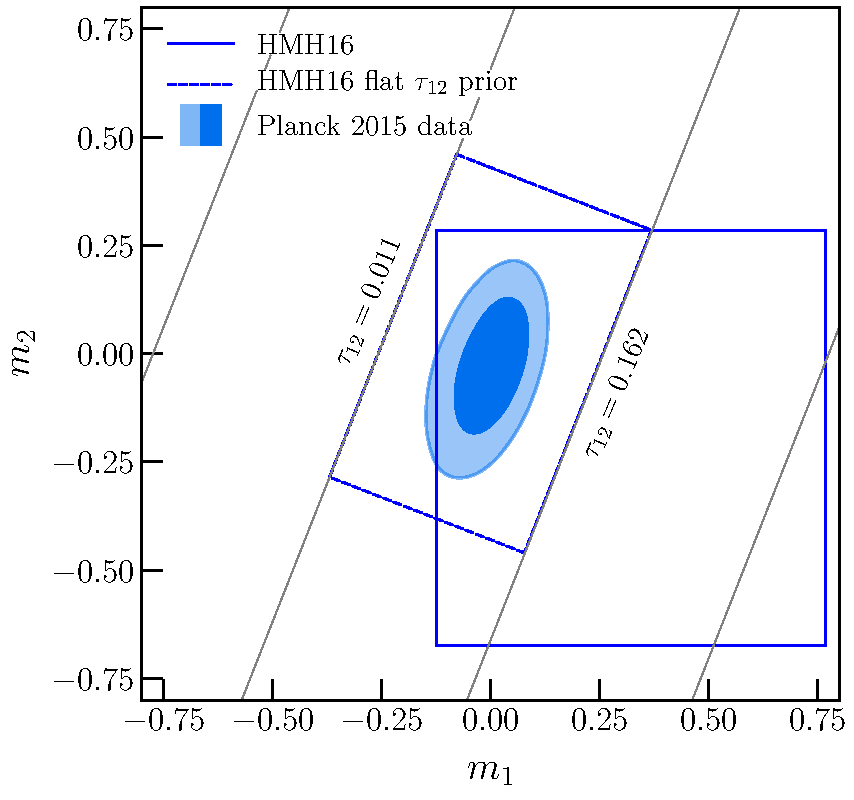
\includegraphics[width=0.9\columnwidth]{paper/plots/plot_rotated_box_flat_tau_prior_fac_0p8.pdf}
          \caption
          {[Placeholder right now (Planck 2015 plot)] Priors on the $m_1-m_2$ parameter space: the original HMH16 prior (inset square, solid lines) and a prior that is flat in
          both $\tau_{12}$ and $m_1-m_2$ (rotated rectangle, dashed lines) whose sides are aligned with lines of
          constant $\tau_{12}$ (light gray lines).   The HMH16 prior allows more parameter space at high vs low $\tau_{12}$ but this
          is not relevant since the data constraints (ellipses) exclude this region.  In the allowed region, the only difference is that the HMH16 prior clips the low $m_1$ edge of the allowed region due to physicality and the assumption that reionization occurs at
          $z\ge 6$. [add in text the comparison of priors, and how tau is not biased, and for KDE physical models determine the priors]}  \label{fig:prior_box}
\end{figure}

[Text: recap our appendix from Planck 2015]

[Text: compare with Planck 2015 our PC results]

[Text: statement that zmax = 50 and zmax = 30 are consistent, there is no evidence for high-redshift ionization for $z>30$.]

[Text: make a point that tanh misses high-z again, compare to PCs using the tau($>z$) plot tanh vs PCs.]

[Table: insert table of mean and covariance matrix for the PC components?]

[Plot: add plot for tau(>z) contours for the 2 parameter model vs PC; direct integration first]

\begin{figure}[ht]
\includegraphics[width=0.45\textwidth]{results/direct_mcmc/pl18_plots_zmax30/plot_pub_tau_gtz_dz_0p1_pl18_pc_zmax30_pliklite_post_0930_and_pl18_pc_zmax30_pliklite_srollv2_0930.pdf}
\caption{[placeholder] PC chains for zmax = 30. Planck 2018 srollv2 likelihood vs Planck 2015).
}
\label{fig:}
\end{figure}

\begin{figure}[ht]
\includegraphics[width=0.45\textwidth]{results/direct_mcmc/pl18_plots_zmax30/plot_pub_tau_gtz_dz_0p1_pl18_pc_zmax30_pliklite_post_0930_and_pl18_pc_zmax30_pliklite_srollv2_0930.pdf}
\caption{PC chains for zmax = 30. Planck 2018 original lowE vs srollv2 likelihood (plik\_lite\_TTTEEE + lowl + simall\_EE vs plik\_lite\_TTTEEE + lowl + sroll2\_EE).
}
\label{fig:}
\end{figure}

\begin{figure}[ht]
\includegraphics[width=0.45\textwidth]{results/direct_mcmc/pl18_plots_zmax30/plot_pub_tau_gtz_dz_0p1_pl18_pc_zmax30_pliklite_srollv2_0930_and_pl18_pc_zmax50_pliklite_srollv2.pdf}
\caption{Comparing zmax = 30 and 50 PC chains using Planck 2018 original lowE likelihood (plik\_lite\_TTTEEE + lowl + sroll2\_EE). Note that the zmax = 30 uses 5 PCs, whereas the zmax = 50 chains uses 7 PCs. .
}
\label{fig:}
\end{figure}

%Optional
\begin{figure}[ht]
\includegraphics[width=0.5\textwidth]{results/direct_mcmc/pl18_plots_zmax30/plot_pub_tau_gtz_dz_0p1_pl18_pc_zmax30_plikfull_and_pl18_tanh_post_plikfull.pdf}
\caption{PC zmax = 30 vs tanh chains with plik\_full\_TTTEEE for the high-l likelihood.
}
\label{fig:}
\end{figure}


\begin{figure}
\includegraphics[width=0.40\textwidth]{plots/plot_tau_gtz.pdf}
\caption{...
}
\label{fig:}
\end{figure}


\begin{figure}
\includegraphics[width=0.40\textwidth]{plots/pl18_pc_zmax30_pliklite_srollv2_1015_tau_posterior_fraccov_1p0_burnin_10000_yes_norm_gaussian0p1_0p12_0p14.pdf}
\caption{...
}
\label{fig:}
\end{figure}


\subsection{Comparison with Previous Results}

[Text: compare with Planck official results]

[Text: comment that Planck tau(15,30) constraints are too stringent (flex knots). Compare to ours. Point out why.]

[Text: compare with Planck official results, PCs (add comments on priors), FlexKnots]

[*Text (maybe in another section): make a point that dz = 0.5 for tanh may not be sufficient for experiments after Planck. This was for higher tau, so transition happens at higher redshift. Now tau is much lower.]

%%%%%%%%%%%%%%%%%%%%%%%%%%%%%%%%%%%%%%%%%%%%

\section{Effective Likelihood}
\label{sec:effective_likelihood}

\subsection{Code description}
\label{sec:code}

\subsection{Example 1: tanh model}
\label{sec:example1}

[to be reworded]
In Fig.~\ref{fig:reion_models}, we show the fiducial ionization history (thick blue) and contrast it with
the standard approach of CAMB (thin black) that takes hydrogen and singly ionized helium reionization to be given by
the tanh form
 \begin{equation}
x_e^{\rm true}(z) = \frac{1+f_{\rm He}}{2}\left\{  1+ \tanh\left[ \frac{y(z_*)-y(z)}{\Delta y} \right] \right\},
 \label{eqn:tanh}
 \end{equation}
 with $y(z)=(1+z)^{3/2}$, $\Delta y=(3/2)(1+z)^{1/2}\Delta z$, and $\Delta z = 0.5$.  We take here $z_*= 9.85$, corresponding the chain maximum likelihood (ML) model ($\tau = 0.0765$) from \S \ref{sec:MCMC},  for illustrative purposes.   Projected onto 5 PCs and resummed into $x_e(z)$, Eq.~(\ref{eq:mmutoxe}) yields a poor reconstruction of the ionization history itself.
 Nonetheless as we shall see in Fig.~\ref{fig:clee}, the PC decomposition provides an 
 excellent representation of the polarization power spectrum.
 

\subsection{Example 2: high-z model}
\label{sec:example2}
[rewording needed]
Our example is a two-step model 
 \bea
x_e^{\rm true}&(z)&\,= \frac{1+f_{\rm He} - \xemin}{2}\left\{  1+ \tanh\left[ \frac{y(z_{\rm re})-y(z)}{\Delta y} \right] \right\} \notag \\
&+& \frac{\xemin - x_e^{\rm rec}}{2}\left\{  1+ \tanh\left[ \frac{z_{\rm t}-z}{\Delta z_{2}} \right] \right\} + x_e^{\rm rec},
 \label{eqn:tanh_highz}
 \eea
where $y(z)=(1+z)^{3/2}$, $\Delta y=(3/2)(1+z)^{1/2}\Delta z_1$, with $\Delta z_1 = 0.25$ instead of the usual $\Delta z_1 = 0.5$,
to provide sharper distinctions between the two steps.
We choose the second step to have $z_{\rm t}=28$  and  $\Delta z_2 = 1.0$  to illustrate below
how the 5 PC analysis with $\zmax=30$ represents the same model.  Here $x_e^{\rm rec}$ is the ionization history from recombination only.
The canonical tanh model is essentially recovered in the limit $\xemin$ approaches the negligible $x_e^{\rm rec}$.  Therefore the double
step model adds a single parameter to control the high-$z$ ionization plateau for $z_{\rm re} \lesssim z \lesssim z_t$.   We show an example
of the two-step model in Fig.~\ref{fig:two_step_model}.


\begin{figure}
\includegraphics[width=0.5\textwidth]{results/cosmomc_kde/taulo_prior_test/plot_xez_taulo_0p04_tauhi_0p02.png}
\caption{Testing \taulo prior -- Full $x_e(z)$ of the model (\taulo, \tauhi) = (0.04, 0.02) shown in the Fig.~\ref{fig:taulo_prior_test_cl}. 
}
\label{fig:two_step_model}
\end{figure}

\begin{figure}
\includegraphics[width=0.5\textwidth]{results/cosmomc_kde/taulo_prior_test/plot_cls_taulo_0p04_tauhi_0p02.png}
\caption{Testing \taulo prior -- testing that \taulo $\geq$ 0.04 as \taulo prior is OK, by calculating $\chi^2$ between $C_l$ from full $x_e(z)$ vs PC decomposition of the model (\taulo, \tauhi) = (0.04, 0.02). 
The $\chi^2 = \sum_{2}^{l_{\rm max}} (\Delta C_l^{EE})^2 / \mathrm{Cov}_l = 0.03$ where $\mathrm{Cov}_l = 2 (C_l^{EE})^2/(2l+1)$. } 
\label{fig:taulo_prior_test_cl}
\end{figure}



\begin{figure}
\includegraphics[width=0.5\textwidth]{results/direct_mcmc/two_parameter_model/tauhi_taulo_chains/pl18_tanh_highz_test2_run1_tri.png}
\caption{Direct MCMC chains of the two-parameter model with \tauhi and \taulo: triangle plot of \tauhi and \taulo. The marginalized 1D constraints are \taulo = $0.0516 \pm 0.0076$, \tauhi = $0.0100 \pm   0.0066$. The ML model is \taulo = 0.0543 and \tauhi = 0.0054 corresponding to $z_{\rm re} = 7.68$ and $x_{e, \mathrm{min}} = 0.021$.
}
\label{fig:two_parameter_model_2D_plot}
\end{figure}


\section{Conclusion}
\label{sec:conclusion}


\bibliography{rei.bib}

\appendix

\section{Outline (in progress)}

\begin{enumerate}
    \item{Intro}
        \begin{enumerate}
            \item 1st paragraph: CMB, reionization, why important
            \item discuss modeling of ionization history in CMB inference, tanh vs PCs (fail to capture high-z; PC captures complete parameter space), mention flex knots/other methods; cite previous PC works.
            \item give context about Planck final results; latest srollv2 likelihood, important to harness all information available, PC allows us to do that and turn into an effective likelihood.
            \item this is what we did: we obtain PC results for Planck 2018, and turn PC chains into a effective likelihood for ionization history: highlight key points like fast inference, entire model space up to zmax 30, code publicly available.
            \item we also compared to Planck official results, which is over stringent at high z, which gives additional motivations for using this likelihood; verified no hint of ionization at z>30; state any additional results.
            \item break down of sections.
        \end{enumerate}

	\item{Background}
		\begin{itemize}
			\item{Reionization Principal Components}	
			\item{Kernel Density Estimate}
		\end{itemize}
	\item{Planck 2018 PC results:\\
		- can discuss discrepancy here on high-redshift tau($>$15) constraints.\\
		- compare with our own 2015 PC results
		- zmax = 30 vs 50}
	\item{Effective Likelihood}
		\begin{itemize}
			\item{Code Description}
			\item{Examples - one and two parameter models}
		\end{itemize}
	\item{Discussion}
		
\end{enumerate}


\end{document}
